% siminos/presentations/kittens/kittens.tex        pdflatex kittens
% $Author: predrag $ $Date: 2019-01-09 08:42:06 -0500 (Wed, 09 Jan 2019) $

% when you get      LaTeX Error: Command \block already defined.
%                   l.512 \newcommand{\block}[1]{\ensuremath{#1}}
% press [Enter] once

%  started with siminos/presentations/GTmath18/GTmath18.tex 2018-03-02
%  started with siminos/presentations/KITP17/UCSB17.tex     2017-01-26
%  started with siminos/presentations/Israel16/Israel16.tex 2016-08-17
%  started with siminos/presentations/GTmap16/GTmap16.tex   2016-08-17
%  started with talks/predrag/NBI16/NBI16.tex               2016-04-25
%  started with talks/predrag/RoySoc16/RoySoc16.tex         2016-04-25

\input ../../inputs/layoutBeamer
\usepackage[font=scriptsize, labelfont=bf]{caption}
\usepackage[
    backend=biber,  %bibtex,
    sorting=nyt,
    %refsection=chapter,
    %citereset=chapter,
    style=numeric, %alphabetic, % %style=authoryear,
    natbib=true,
    style=phys, % aps
    biblabel= brackets, % superscript, %
    articletitle=false, % true,  % false, % aps
    %chaptertitle=true,  % aip;  % false, % aps
    pageranges = true , % aip: the full range
             % = false, % aps: only the first page being printed
    sortlocale=en_US,
    firstinits=true,
    url=false, %true,  %
    doi=false, %true,
    eprint=false
]{biblatex}
\addbibresource{../../bibtex/siminos.bib}
\setbeamerfont{footnote}{size=\tiny}
\input ../../inputs/def % no edits, always from dasbuch/book/inputs
\input ../../inputs/defsBeamer
\renewcommand{\Ssym}[1]{{\ensuremath{m_{#1}}}}    % Boris
% \newcommand{\Ssym}[1]{{\ensuremath{s_{#1}}}}  % ChaosBook
\newcommand{\D}{\mathcal{D}}
\newcommand{\gd}{\mathsf{g}}

\begin{document}
\title{
{\huge \catlatt}
    \\
{the simplest chaotic field theory}
}
\author{P. Cvitanovi\'c}
\author[Cvitanovi\'c]
{
  \textcolor{green!50!black}{
  {Predrag~Cvitanovi\'c,
  Han Liang
   \\
  Matt Gudorf,
  Nazmi Burak Budanur,
        Li Han,
        Rana Jafari,
		Adrien K. Saremi,
  and
  Boris Gutkin
  }	%\inst{1}
  }
}
\institute
{
%  \inst{1}%
ChaosBook.org/overheads/spatiotemporal   ~ notes
\\
                Georgia Tech
 }
\date{January 4, 2019}

\begin{frame}
  \titlepage
\end{frame}


\section[what this talk is about]
 {what this talk is about}

\begin{frame}{overview}
\begin{enumerate}
              \item {\Large
what this is about
                  }\textcolor{gray}{\small
%\\{\scriptsize \em
% (to skip the motivational blah blah: go to part \textcolor{red}{\ref{spacetimeFT}})
% }
              \item
a modern cat
              \item
\catlatt\
              \item
bye bye, dynamics
                    }
            \end{enumerate}
\end{frame}


\section[dynamics in $\infty$ dimensions]
{dynamics in $\infty$ dimensions}

\begin{frame}{an example of spacetime turbulent field configuration}
\begin{block}{complex Ginzburg-Landau}
  \includegraphics[width=0.515\textwidth] %,height=0.5\textheight,clip=true]
  {cGLdefturbabs}
  \hfill
  (will return to this)
\end{block}

{\footnotesize
[horizontal] space $\ssp \in [-L/2,L/2]$
\qquad
{[up]} time evolution
}

\hfill {\scriptsize \color{orange} codeinthehole.com/static/tutorial/coherent.html}
\end{frame}

\begin{frame}{an example of spacetime turbulent field configuration}
\begin{block}{\KS}
  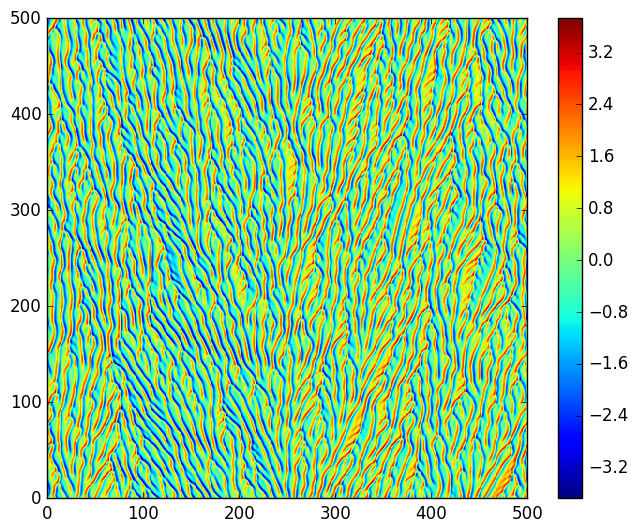
\includegraphics[width=.7\textwidth]{MNG_uu500b500}
%  \includegraphics[width=0.6\textwidth] %,height=0.5\textheight,clip=true]
%  {ks_largeL_cbar_200} %{ksevol-fig} %{ks_largeL_cbar}
  \hfill
\end{block}

{\footnotesize
[horizontal] space $\ssp \in [0,L]$
\qquad
{[up]} time evolution
}
\end{frame}

\begin{frame}{describe this!}
now and forever you will be able to distinguish
\\
 a \KS\ field configuration vs.
 \\
a complex Ginzburg-Landau field configuration

\bigskip
we need the corresponding
\begin{block}{alphabets of spatiotemporal patterns} % (chronotopes)}
and grammars of admissible ways of joining them
\end{block}
\vfill

{\Large \catlatt} \hfill teaches us that
\end{frame}

\begin{frame}{complex Ginzburg-Landau field configuration}
\begin{block}{goal : enumerate nearly recurrent patterns } %chronotopes}
  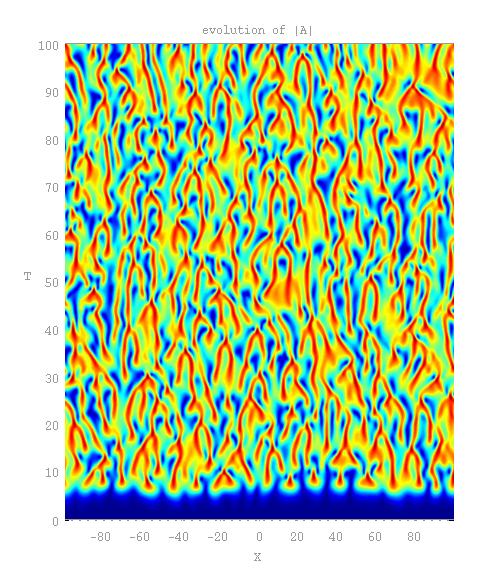
\includegraphics[width=0.4635\textwidth]{cGLdefturbabs}%
~~\raisebox{+3.33ex}[5.5ex][4.5ex]
		 {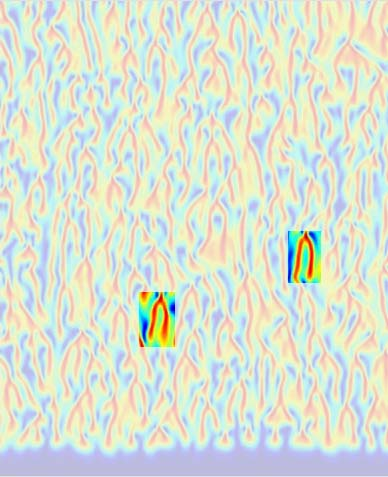
\includegraphics[width=0.36\textwidth]{cGLdefturbclip}}
\end{block}

{\footnotesize
[left-right] space $\ssp \in [-L/2,L/2]$
\qquad
{[up]} time $t\in [0,\period{}]$
}
\end{frame}

\begin{frame}
    \frametitle{\KS\  field configuration}
\begin{block}{goal : enumerate nearly recurrent patterns } %chronotopes}
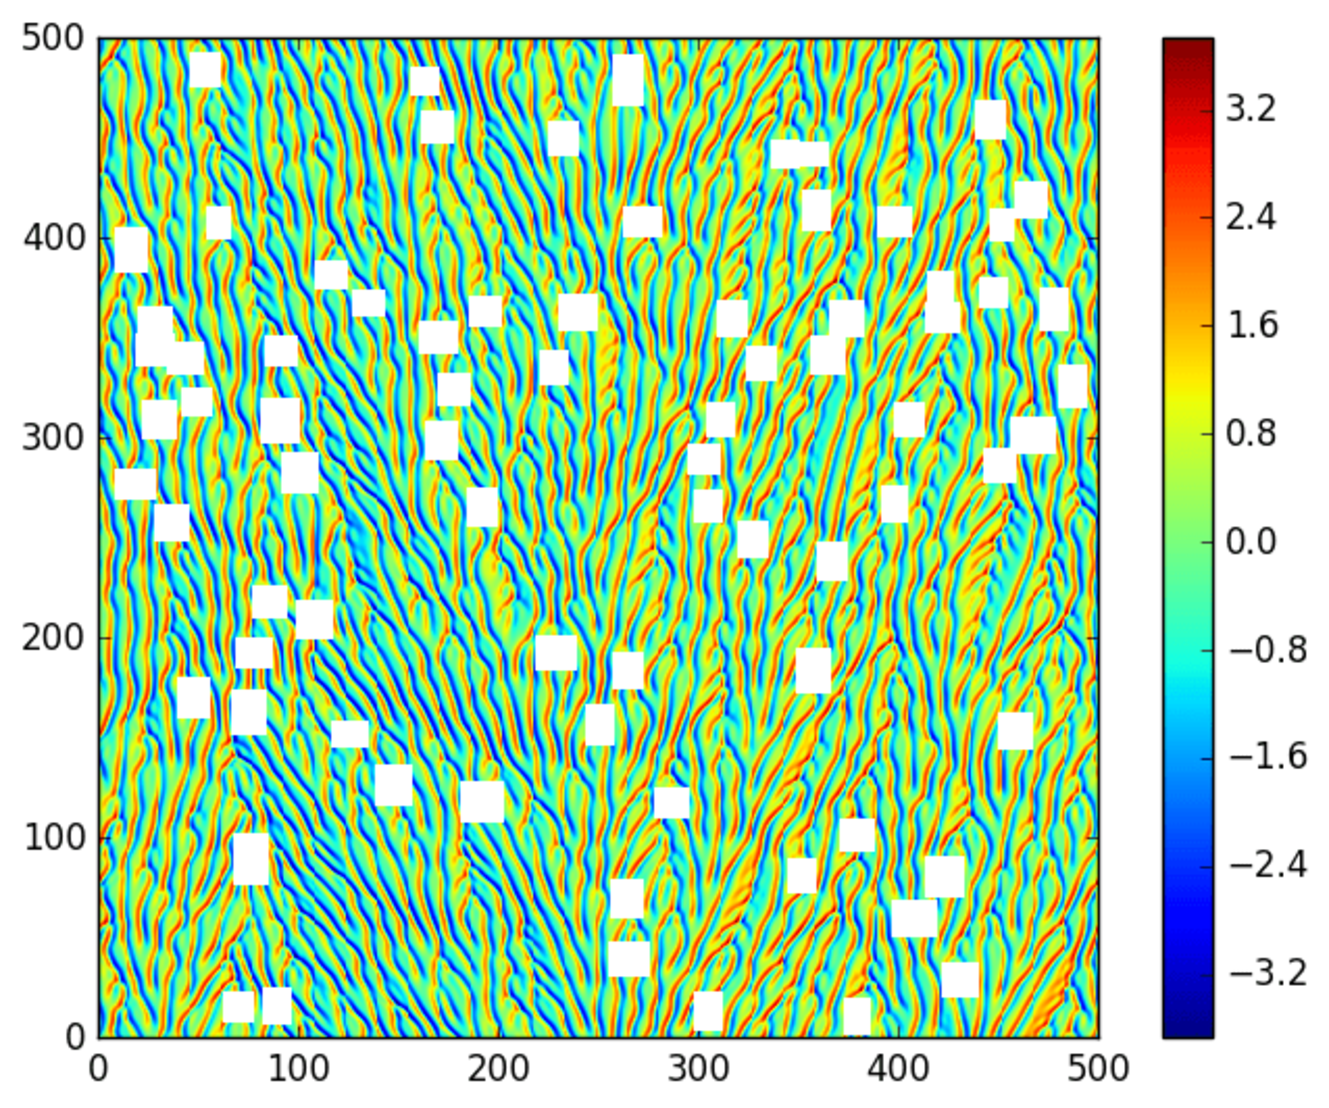
\includegraphics[width=.48\textwidth]{MNG_uu500b500co}
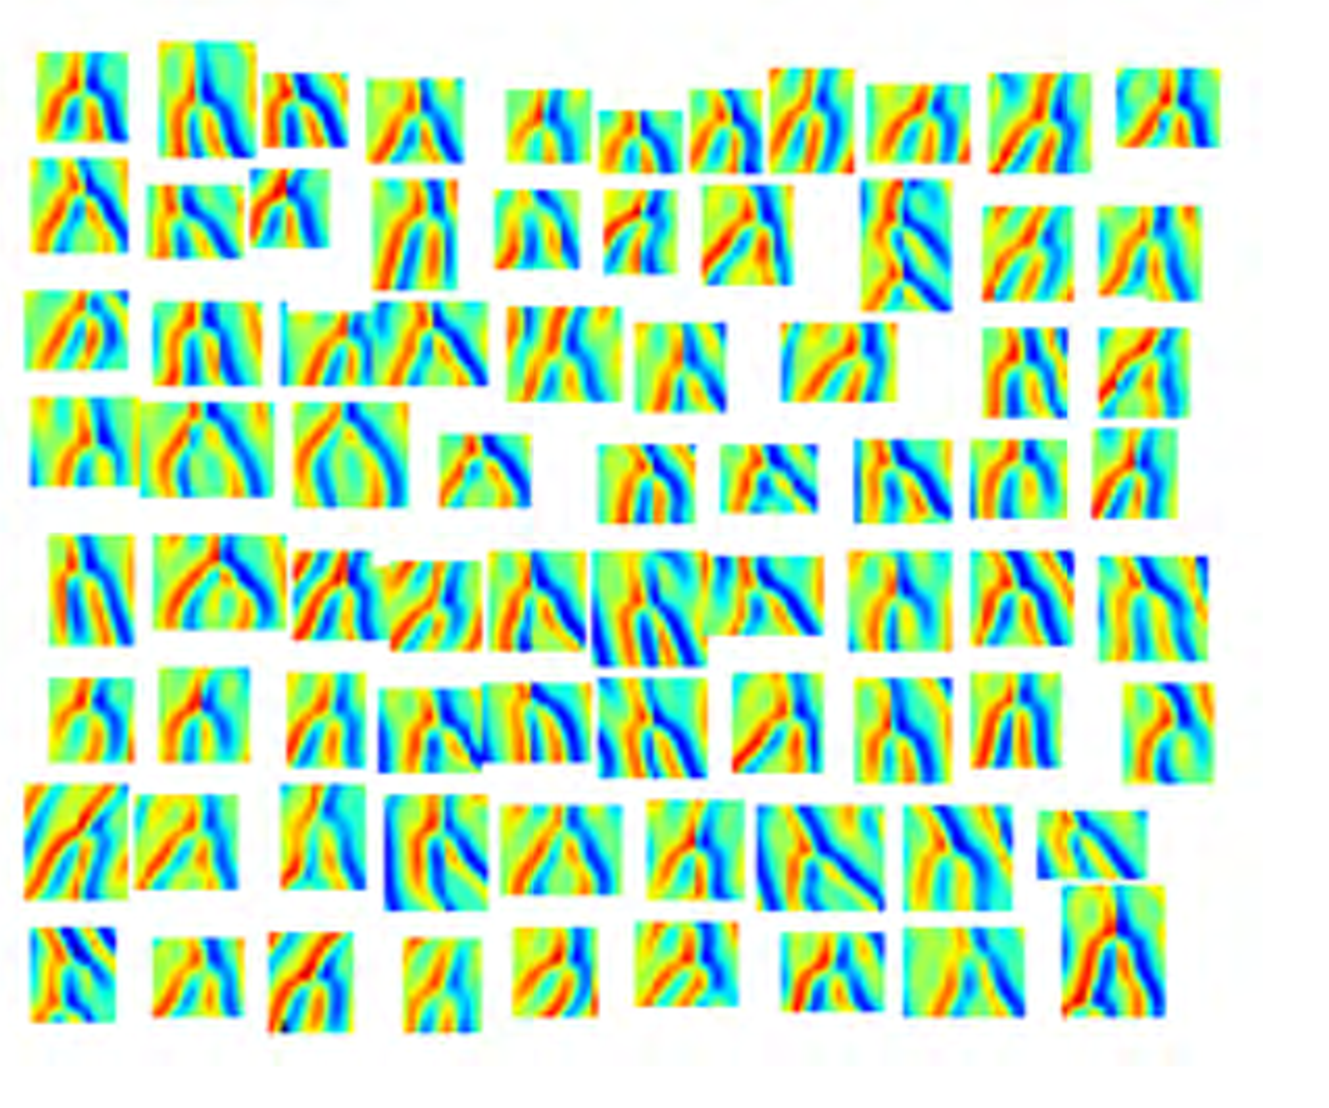
\includegraphics[width=.48\textwidth]{cutouts}
\end{block}
\end{frame}

\begin{frame}{the simplest of chaotic field theories ?}
a description of \\
the admissible \KS, \\
complex Ginzburg-Landau
or Navier-Stokes \\
field configurations is still out of our reach

\bigskip
\begin{block}{we need a simple exact model to hone our intuition}
\bigskip

{\Large \catlatt} \hfill does that
\end{block}
\end{frame}

\begin{frame}{example : the simplest 1D dynamical system}
    \begin{block}{Bernoulli shift map : linear mod 1}
% ChaosBook {fig:BernPartExam}
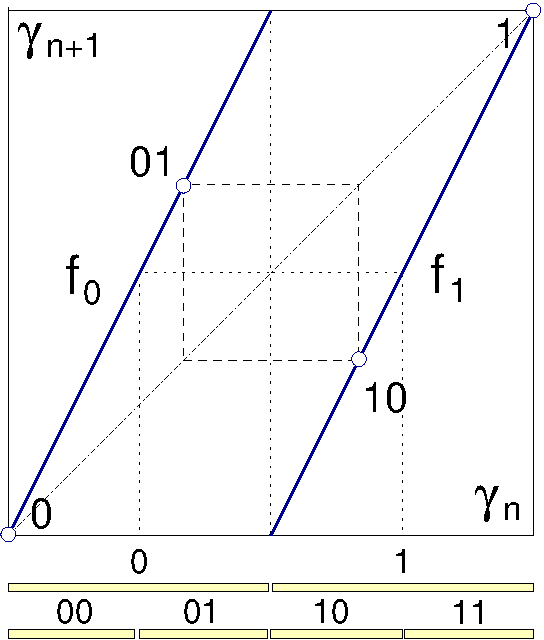
\includegraphics[width=0.33\textwidth]{BernPart}
    \end{block}

\bigskip

The $\cl{}=2$ and 4 intervals \statesp\ partitions,
\\
together with the
fixed points \cycle{0}, \cycle{1} and the 2-cycle \cycle{01}.
\bigskip

makes precise the sense in which

\hfill deterministic chaos is a coin flip
\end{frame}

\section[spacetime field theory]
 {spacetime field theory}
\label{spacetimeFT}

\begin{frame}{}
\begin{enumerate}
              \item \textcolor{gray}{\small
what this is about
                  }
              \item {\Large
a cool cat
                  }\textcolor{gray}{\small
              \item
\catlatt\
              \item
bye bye, dynamics
                    }
            \end{enumerate}
\end{frame}

\begin{frame}{a field theory in one spacetime dimension (1-torus)}
start with

\bigskip

\begin{block}{cat map in $1$ spacetime dimension}
then generalize to

\bigskip

$d$ spacetime dimensional {\Large \catlatt}
\end{block}

\vfill

\begin{itemize}
  \item cat map in Hamiltonian formulation
  \item cat map in Lagrangian formulation
\end{itemize}
\end{frame}

\begin{frame}{1. the traditional cat map}
\vfill

\begin{center}
{\huge Hamiltonian formulation}
\end{center}

\vfill
\end{frame}


\begin{frame}{example of a ``small domain dynamics'' : kicked rotor}
an electron circling an atom, subject to

a discrete time
sequence of angle-dependent kicks $F(x_{t})$

\hfill  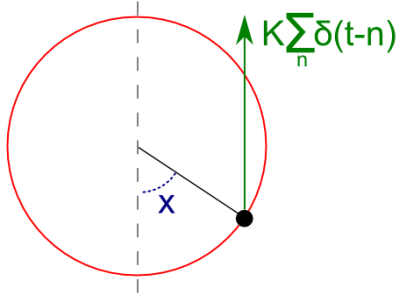
\includegraphics[width=0.33\textwidth]{kicked-rotor}

\begin{block}{Taylor, Chirikov and Greene  standard map}
\bea
x_{t+1} &=& x_{t}+p_{t+1} \qquad  \mod 1, \continue
p_{t+1} &=& p_{t} + F(x_{t})             \nnu
\eea
\end{block}

\medskip

\hfill $\to$ {\color{red}
chaos in Hamiltonian systems}
\end{frame}

\begin{frame}{the simplest example : a cat map evolving in time}

force
\(
 F(x) = Kx
\)
linear in the displacement $x$
\,,\;
$K\in\integers$
\bea
x_{t+1} &=& x_{t}+p_{t+1} \quad  \mod 1
        \continue
p_{t+1} &=& p_{t} + K x_{t} \qquad  \mod 1 \nnu
\eea
 \textcolor{red}{C}ontinuous
 \textcolor{red}{A}utomorphism of the
 \textcolor{red}{T}orus, or

\begin{block}{Hamiltonian cat map}
a linear, area preserving map of a 2-torus onto itself
 \[
 \left(\begin{array}{c}
   x_{t+1}  \\
   p_{t+1}
  \end{array} \right )=
  A \left(\begin{array}{c}
   x_t  \\
   p_t
  \end{array} \right )\quad \mod 1
\,,\qquad
A = \left (
\begin{array}{cc}
s-1 & 1 \\
s-2 & 1 \\
\end{array}
    \right )
 \] %\ee{eq:CatMapIntr}
\end{block}
for integer ``stretching''
$s=\tr{A} > 2$ the map is \\ hyperbolic $\to$ a
fully chaotic Hamiltonian dynamical system
\end{frame}

\begin{frame}{$s=3$ cat map Adler-Weiss generating partition}
%%%%%%%%%%%%%%%%%%%%%%%%%%%%%%%%%%%%%%%%%%%%%%%%%%%%%%%%%%%%%
% PC 2018-02-09 from siminos/cats/catAdlerWeiss.tex
% \caption{\label{fig:PVAdlerWeissB}
\begin{center}
            \begin{minipage}[c]{0.23\textwidth}\begin{center}
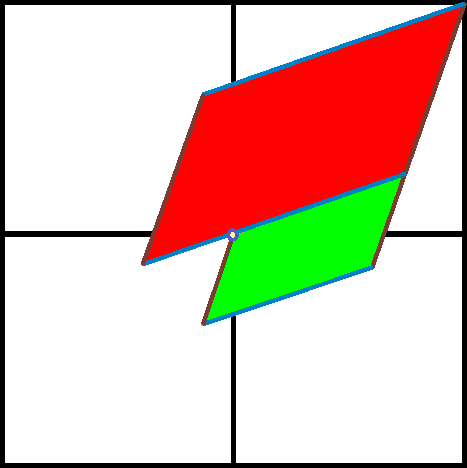
\includegraphics[width=1.0\textwidth]{PVAdlerWeissB-a}%\\(a)
            \end{center}\end{minipage}
            \hspace{5ex}
            \begin{minipage}[c]{0.46\textwidth}\begin{center}
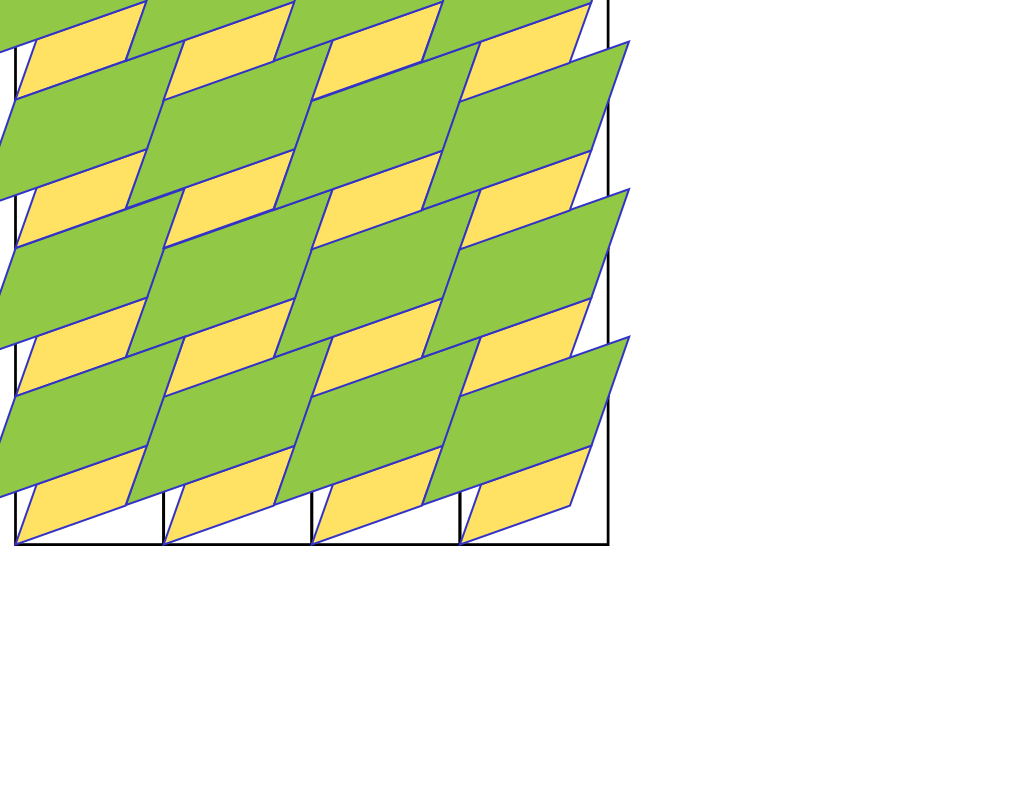
\includegraphics[width=1.0\textwidth]{PCLect13p12}%\\(b)
            \end{center}\end{minipage}
\end{center}
%%%%%%%%%%%%%%%%%%%%%%%%%%%%%%%%%%%%%%%%%%%%%%%%%%%%%%%%%%%%%%%
generating partition
of the unit torus with \\
rectangles $\pS_A$ (red) and $\pS_B$ (green)
% for the Percival--Vivaldi cat map,

borders given by the cat map \\
stable (blue) and
unstable (dark red) manifolds.

\medskip

[right frame] it is a plane tiling % (sorry about colors)
\end{frame}

\begin{frame}{cat map generating partition}
%%%%%%%%%%%%%%%%%%%%%%%%%%%%%%%%%%%%%%%%%%%%%%%%%%%%%%%%%%%%%
% PC 2018-02-09 from siminos/cats/catAdlerWeiss.tex
% \caption{\label{fig:PVAdlerWeissB}
\begin{center}
            \begin{minipage}[c]{0.23\textwidth}\begin{center}
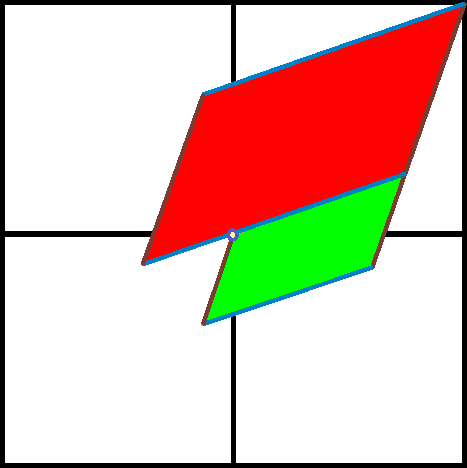
\includegraphics[width=1.0\textwidth]{PVAdlerWeissB-a}\\(a)
            \end{center}\end{minipage}
            \begin{minipage}[c]{0.23\textwidth}\begin{center}
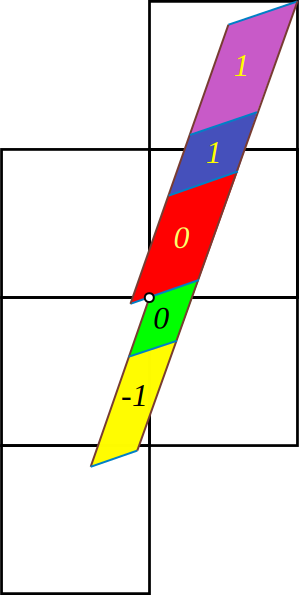
\includegraphics[width=1.0\textwidth]{PVAdlerWeissB-b}\\(b)
            \end{center}\end{minipage}
            \begin{minipage}[c]{0.23\textwidth}\begin{center}
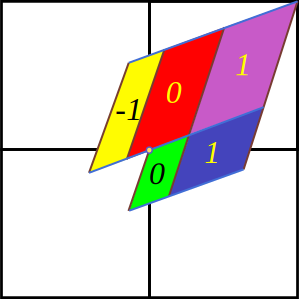
\includegraphics[width=1.0\textwidth]{PVAdlerWeissB-c}\\(c)
            \end{center}\end{minipage}
\end{center}
%%%%%%%%%%%%%%%%%%%%%%%%%%%%%%%%%%%%%%%%%%%%%%%%%%%%%%%%%%%%%%%
(b)
mapped step forward in time, the rectangles are stretched along the
unstable direction and shrunk along the stable direction

(c) sub-rectangles
$\pS_j$ that have to be translated back into the partition are indicated by
color and labeled by their lattice translations
$\Ssym{j}\in\A=\{\underline{1},0,1\}$
%%%%%%%%%%%%%%%%%%%%%%%%%%%%%%%%%%%%%%%%%%%%%%%%%%%%%%%%%%%%%%%
\end{frame}

\begin{frame}{cat map generating partition}
%%%%%%%%%%%%%%%%%%%%%%%%%%%%%%%%%%%%%%%%%%%%%%%%%%%%%%%%%%%%%
% PC 2018-02-09 from siminos/cats/catAdlerWeiss.tex
% \caption{\label{fig:PVAdlerWeissB}
\begin{center}
            \begin{minipage}[c]{0.23\textwidth}\begin{center}
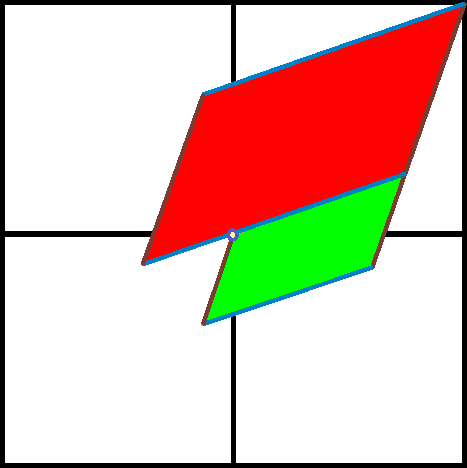
\includegraphics[width=1.0\textwidth]{PVAdlerWeissB-a}\\(a)
            \end{center}\end{minipage}
%            \begin{minipage}[c]{0.23\textwidth}\begin{center}
%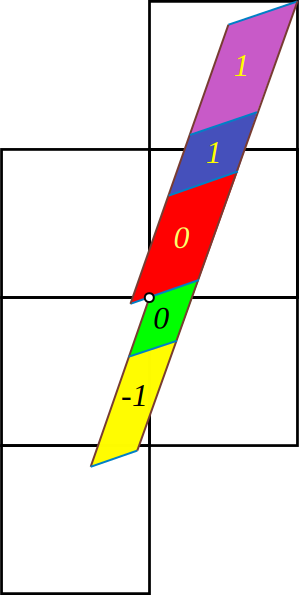
\includegraphics[width=1.0\textwidth]{PVAdlerWeissB-b}\\(b)
%            \end{center}\end{minipage}
            \begin{minipage}[c]{0.23\textwidth}\begin{center}
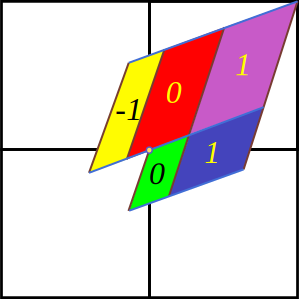
\includegraphics[width=1.0\textwidth]{PVAdlerWeissB-c}\\(c)
            \end{center}\end{minipage}
            ~~~
            \begin{minipage}[c]{0.09\textwidth}\begin{center}
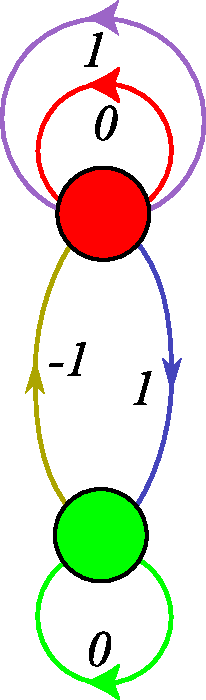
\includegraphics[width=1.0\textwidth]{PVAWMarkovCol}\\(d)
            \end{center}\end{minipage}
\end{center}
%%%%%%%%%%%%%%%%%%%%%%%%%%%%%%%%%%%%%%%%%%%%%%%%%%%%%%%%%%%%%%%
(c)
sub-rectangles $\pS_j$ yield a generating partition, with
\\
(d)
the finite grammar given by the finite {\markGraph}.

\medskip

The nodes
refer to the rectangles $A$ and $B$, \\
the five links correspond to the five sub-rectangles \\
induced by one step forward-time dynamics.
%\footnote{For details, see ChaosBook.org}

\bigskip {\scriptsize \em
\hfill \textcolor{green}{this construction is new, not in literature}
         }

%%%%%%%%%%%%%%%%%%%%%%%%%%%%%%%%%%%%%%%%%%%%%%%%%%%%%%%%%%%%%%%
\end{frame}

\begin{frame}{cat map Perron-Frobenious operator}
%%%%%%%%%%%%%%%%%%%%%%%%%%%%%%%%%%%%%%%%%%%%%%%%%%%%%%%%%%%%%
% PC 2018-02-09 from siminos/cats/catAdlerWeiss.tex
% \caption{\label{fig:PVAdlerWeissB}
\begin{center}
            \begin{minipage}[c]{0.23\textwidth}\begin{center}
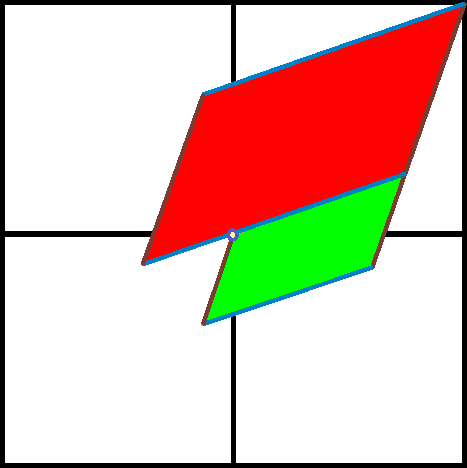
\includegraphics[width=1.0\textwidth]{PVAdlerWeissB-a}
            \end{center}\end{minipage}
            \begin{minipage}[c]{0.23\textwidth}\begin{center}
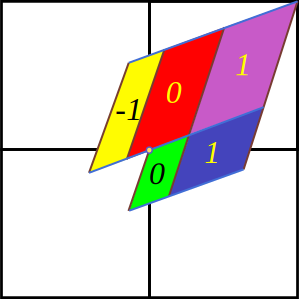
\includegraphics[width=1.0\textwidth]{PVAdlerWeissB-c}
            \end{center}\end{minipage}
            ~~~
            \begin{minipage}[c]{0.09\textwidth}\begin{center}
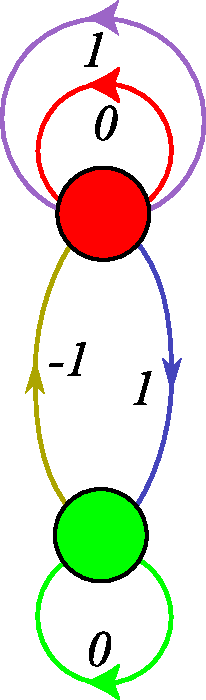
\includegraphics[width=1.0\textwidth]{PVAWMarkovCol}
            \end{center}\end{minipage}
\end{center}
%%%%%%%%%%%%%%%%%%%%%%%%%%%%%%%%%%%%%%%%%%%%%%%%%%%%%%%%%%%%%
% PC 2018-02-09 from siminos/spatiotemp/chapter/blogHL.tex
the two-rectangle partition has [2$\times$2] Markov
matrix, \\ where one sums over all admissible transitions:
\bea
\left[\begin{array}{c} \phi'_A \\ \phi'_B \end{array}\right]
&=& L\phi =
\left[
\begin{array}{cc}
 L_{A{}^0\!A}+L_{A{}^1\!A} & L_{A{}^{\underline{1}}\!B} \\
 L_{B{}^1\!A} & L_{B{}^0\!B} \\
\end{array}
\right]
\left[\begin{array}{c} \phi_A \\ \phi_B \end{array}\right]
    \continue       %{2rectTransfMatrEq}
L &=&
\frac{1}{\ExpaEig}
\left[\begin{array}{cc}
 2          & \ExpaEig-2 \\
 \ExpaEig-1 & 1          \\
\end{array}\right]
\nnu %\label{2rectTransfMatrEq1}
\eea
%%%%%%%%%%%%%%%%%%%%%%%%%%%%%%%%%%%%%%%%%%%%%%%%%%%%%%%%%%%%%%%
\end{frame}

\begin{frame}{cat map dynamical zeta function}
%%%%%%%%%%%%%%%%%%%%%%%%%%%%%%%%%%%%%%%%%%%%%%%%%%%%%%%%%%%%%
% PC 2018-02-09 from siminos/cats/catAdlerWeiss.tex
% \caption{\label{fig:PVAdlerWeissB}
\begin{center}
            \begin{minipage}[c]{0.23\textwidth}\begin{center}
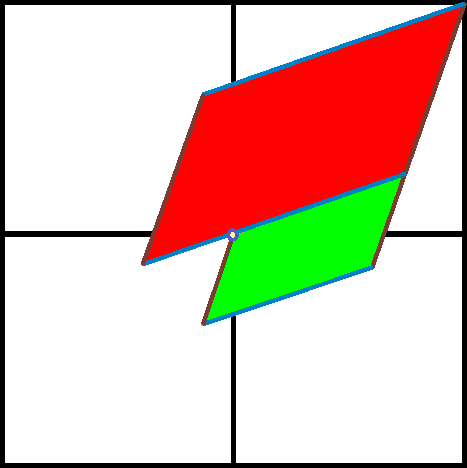
\includegraphics[width=1.0\textwidth]{PVAdlerWeissB-a}
            \end{center}\end{minipage}
            \begin{minipage}[c]{0.23\textwidth}\begin{center}
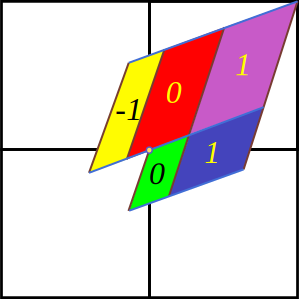
\includegraphics[width=1.0\textwidth]{PVAdlerWeissB-c}
            \end{center}\end{minipage}
            ~~~
            \begin{minipage}[c]{0.09\textwidth}\begin{center}
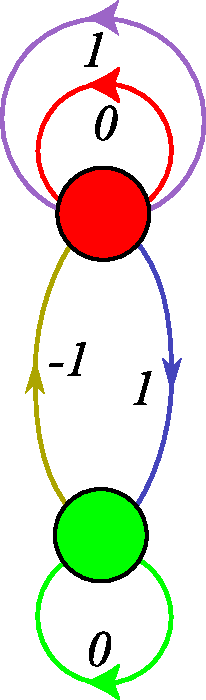
\includegraphics[width=1.0\textwidth]{PVAWMarkovCol}
            \end{center}\end{minipage}
\end{center}
%%%%%%%%%%%%%%%%%%%%%%%%%%%%%%%%%%%%%%%%%%%%%%%%%%%%%%%%%%%%%
% PC 2018-02-09 from siminos/spatiotemp/chapter/blogHL.tex
every long-time property of cat maps dynamics is encoded in \\
the Fredholm determinant \\
(topological zeta function\footfullcite{Isola90};
Markov graph determinant)
\[
\det(1-zL) = %2019-01-03 PC no longer understands where
             %           the commented-out version came from....
 % 1-3\frac{z}{\ExpaEig}
 %   -\frac{z^2}{\ExpaEig}(\ExpaEig-3)
 \frac{1 - 3 z + z^2}{(1 - z)^2}
%\label{2rectDetTransfMatr}
\]
%%%%%%%%%%%%%%%%%%%%%%%%%%%%%%%%%%%%%%%%%%%%%%%%%%%%%%%%%%%%%%%

{\Huge \textcolor{red}{solved!}} \hfill every expectation value computable
\end{frame}

\begin{frame}{2. a modern cat map}
\vfill
\begin{center}
{\huge Lagrangian formulation}
\end{center}
\vfill
\end{frame}

\begin{frame}{cat map in Lagrangian form}
replace momentum by velocity
\[
p_{t+1}=(\ssp_{t+1}  - \ssp_{t})/\Delta t
\]
dynamics in $(\ssp_{t},\ssp_{t-1})$  \statesp\
is particularly pretty\footfullcite{PerViv}
\begin{block}{2-step difference equation}
\[
\ssp_{t+1}  -  s \, \ssp_{t} + \ssp_{t-1}
    =
-\Ssym{t}
\] %\ee{eq:CatMapNewton1}
\end{block}
unique integer $\Ssym{t}$
ensures that

\hfill $\ssp_{t}$ lands in the unit interval at time step $t$

\bigskip
nonlinearity : $ \mod 1$ operation, encoded in
\[
\Ssym{t}\in  \A
\,,\quad \A\ = \mbox{ finite alphabet of possible values for } \Ssym{t}
\]
\end{frame}

\begin{frame}{cat map is $d=1$ lattice damped Poisson equation}
\[
 (\Box -s+2)\,\ssp_{t} = \m_t
%    \,, \qquad
\] %\ee{LinearConn}

\vfill

\hfill
\textcolor{red}{did you know that a cat map can be so cool?}
\end{frame}

\begin{frame}{Lagrangian insight : }
no need for explicit partition to derive the zeta function
\end{frame}

\begin{frame}{number of periodic points of a cat map with time period $n$ }
\begin{block}{Lagrangian formulation}
the number of periodic points is
\bea
N_n = \det H_n
 = \prod_{j=0}^{n-1}
             \left[s - 2 \cos\left(\frac{2 \pi j}{n}\right)\right]
%= 2\,T_n(s/2) -2
= \Lambda^n + \Lambda^{-n} - 2
%\,,
%\label{perOrbits:??-2}
\eea
% $T_n(s/2)$ : the Chebyshev polynomial of the first kind
where  $H_n$ is the \po\ Hessian matrix
\end{block}
\begin{block}{Hamiltonian formulation}
the number of periodic points  is
\[
N_n = |\det(A^n - \matId)|
            = \Lambda^n + \Lambda^{-n} - 2
%\, ,
%\label{perOrbits:Isola90-11}
\]
$\Lambda$ : eigenvalue of matrix $A$
\end{block}
\vfill\hfill
equivalent by Hill (1886) formula \quad
\(
|\det(A^n - \matId)| = \det H_n
%\label{catHillform}
\)
\end{frame}

\begin{frame}{cat map \tzeta}
substitute the number of periodic points $N_n$ into the
{\em topological} or {\em Artin-Mazur} zeta func\-tion\footfullcite{ArtMaz65}.
That recovers the previous zeta function
\bea
\zetatop(z)
&=& \exp \left(
    -\sum_{n=1} \frac{z^n}{n} N_n
    \right)
 =  \exp \left[-\sum_{n=1}
                \frac{z^n}{n} (\Lambda^n + \Lambda^{-n} - 2) \right]
\continue
&=& \exp \left[\ln(1 - z \Lambda) + \ln(1 - z \Lambda^{-1}) - 2 \ln(1 - z) \right]
%\continue
%&=& (1 - z \Lambda)^{-1} (1 - z \Lambda^{-1})^{-1} (1 - z)^2
\continue
&=& \frac{(1 - z \Lambda)(1 - z \Lambda^{-1})}{(1 - z)^2}
           =  \frac{1 - s z + z^2}
                  {(1 - z)^2}
%\label{perOrbits:Isola90-13}
\eea

\vfill
{\Huge \textcolor{red}{solved!}} \hfill without any explicit partition
\textcolor{red}{(!)}
\end{frame}

\begin{frame}{that's it! for $d=1$ dimension}
lattice damped Poisson equation
\[
 (\Box -s+2d)\ssp_{z} = \m_z
%    \,, \qquad
\] %\ee{LinearConn}
\hfill solved completely and analytically!
\end{frame}

\begin{frame}{herding cats}
\begin{enumerate}
              \item \textcolor{gray}{\small
what this is about
              \item
a cool cat
                  }
              \item {\Large
\catlatt\
                  }\textcolor{gray}{\small
              \item
bye bye, dynamics
                    }
            \end{enumerate}
\end{frame}

\begin{frame}{next : herding cats in $d$ spacetime dimensions}
start with

\bigskip

\begin{block}{a cat map at each lattice site}
generalize to

\bigskip

$d$ spacetime dimensional {\Large \catlatt}
\end{block}

\vfill

\begin{itemize}
  \item Hamiltonian formulation is awkward, forget about it
  \item Lagrangian formulation is elegant
\end{itemize}
\end{frame}

\begin{frame}{spatiotemporally infinite \catlatt}
%\begin{center}
%\hfill
\includegraphics[width=0.55\textwidth]{spatiotempCat}
\hfill
\includegraphics[width=0.55\textwidth]{DawnBishopCats}
%\end{center}
\end{frame}

\begin{frame}{spatiotemporal cat map - the construction}
consider
a 1 spatial dimension lattice, with field
$\ssp_{nt}$ \\
(the angle of a kicked
rotor ``particle'' at instant $t$, at site $n$)
\begin{block}{require}
\begin{itemize}
\item  each site couples to
its nearest neighbors $\ssp_{n\pm1,t}$
\item  invariance under
spatial translations
\item  invariance under spatial reflections
\item  invariance under the space-time exchange
\end{itemize}
\end{block}

\bigskip

obtain\footfullcite{GutOsi15}
\begin{block}{2\dmn\ coupled cat map lattice}
\[
\ssp_{n,t+1} + \ssp_{n,t-1} - s \, \ssp_{n t} + \ssp_{n+1,t} + \ssp_{n-1, t}
     =-\Ssym{n t}
\] %\ee{eq:CatMapNewton2}
\end{block}
\end{frame}

\begin{frame}{a discrete Euclidean space-time field theory}
write the spatial-temporal differences as discrete derivatives
\begin{block}{Laplacian : in $d=1$ and $d=2$ dimensions}
\(
\Box \ssp_t \;\;\,=\, \ssp_{t+1} - 2\ssp_{t} + \ssp_{t-1}
\)\\ \(
\Box \ssp_{nt} \,=\, \ssp_{n,t+1} + \ssp_{n,t-1}
- 4 \, \ssp_{nt} + \ssp_{n+1,t} + \ssp_{n-1, t}
\)
\end{block}

\medskip

$\to$ the cat map is thus generalized  to
\begin{block}{$d$\dmn\ \catlatt}
\[
 (\Box -s+2d)\ssp_{z} = \m_z
%    \,, \qquad
\] %\ee{LinearConn}

\medskip

\end{block}

\bigskip

where
\(
  \ssp_{z} \in  \mathbb{T}^{1}
    \,, \quad
  \Ssym{z} \in \A
    \mbox{  and  }
  z\in \integers^{d}
\) = lattice site label
\end{frame}

\begin{frame}{discretized linear PDE}
\begin{block}{$d$\dmn\ \catlatt}
{\Large
\[
 (\Box -s+2d)\,\ssp_{z} = \m_z
%    \,, \qquad
\] %\ee{LinearConn}
}
\end{block}

\bigskip

is linear and known as
\begin{itemize}
\item Helmholtz equation if stretching is weak, $s<2d$ \\
(oscillatory sine, cosine solutions)
\item damped Poisson equation if stretching is strong, $s>2d$ \\
(hyperbolic sinches, coshes)
\end{itemize}
the nonlinearity is hidden in the ``source''
\[
  \Ssym{z} \in \A
    \mbox{  at lattice site  }
  z\in \integers^{d}
\]
\end{frame}

\begin{frame}{the simplest of all `turbulent' field theories}
\catlatt
\[
 (\Box -s+2d)\ssp_{z} = \m_z
%    \,, \qquad
\] %\ee{LinearConn}
\bigskip
\hfill can be solved completely and analytically!

\bigskip
\bigskip

Assign to each site $z$ a
letter \Ssym{z}\ from the alphabet $\A$.

\medskip

A particular fixed set
of letters  \Ssym{z}\ (a lattice state)
\[
\Mm= \{\Ssym{z}\} % \in \A \,,\; z\in \integers^d \}
 = \{\Ssym{n_1 n_2 \cdots n_d}\}
\,,
\]
is a complete specification of the corresponding \\
field configuration $\Xx$.
\end{frame}

\begin{frame}{solving $1D$ cat map using Green's functions}
\begin{block}{the Green's function for a period \period{} solution of}
\[
 (\Box -s+2)\ssp_{t} = \m_t
%    \,, \qquad
\] %\ee{LinearConn}

\medskip
\end{block}
\begin{block}{is a Toeplitz matrix $\gd$ that satisfies}
\bea
 (\D \gd)_{tt'}&=&\delta_{nn'}\,, \qquad t,t'\in 0,1,2,\cdots,\period{}-1
% \label{1DGreenFun0} \ee{1DGreenFunDirichlet}
        \continue
   & &  \continue
\D &=&\left(\begin{array}{ccccccc}
 s&-1 & 0 & 0 &\dots &0&-1 \\
-1 &  s&-1 & 0 &\dots &0&0 \\
0 &-1 &  s&-1 &\dots &0 & 0 \\
\vdots & \vdots &\vdots & \vdots & \ddots &\vdots &\vdots\\
0 & 0 & \dots &\dots &\dots  & s&-1 \\
-1 & 0 & \dots &  \dots &\dots&-1 &  s
        \end{array} \right )
\nnu
\eea %ee{3diagToeplitz}
\medskip
\end{block}
\end{frame}


\begin{frame}{examples of spacetime periodic $[3\times3]$ \brick s}
with $z=(\ell t),z'=(\ell' t')\in T^2_{(3,3)}$.

the symbol \brick s and the corresponding field values of two
admissible 2-torus field configurations
\beq
\Mm_1=
\left(
\begin{array}{ccc}
 1 & 0 & 0 \\
 0 & 1 & 0 \\
 0 & 0 & 1 \\
\end{array}
\right)
            \Rightarrow\quad
\Xx_1=\frac{1}{7}
\left(
\begin{array}{ccc}
 3 & 2 & 2 \\
 2 & 3 & 2 \\
 2 & 2 & 3 \\
\end{array}
\right)
\ee{HL2DimensionOrbit1}
\beq
\Mm_2=
\left(
\begin{array}{ccc}
 1 & 0 & 0 \\
 0 & 1 & 2 \\
 0 & 0 & 1 \\
\end{array}
\right)
            \Rightarrow\quad
\Xx_2=\frac{1}{14}
\left(
\begin{array}{ccc}
 8 & 6 & 7 \\
 7 & 9 & 12 \\
 6 & 6 & 9 \\
\end{array}
\right)
\ee{HL2DimensionOrbit2}
\end{frame}

\begin{frame}{insight 1 : how is turbulence described?}
\begin{block}{not by the evolution of an initial state}
exponentially unstable system have finite (Lyapunov) time and
space prediction horizons
\end{block}
but
\bigskip

\begin{block}{by enumeration of admissible field configurations}
and the relative frequency of their occurence
\end{block}
\end{frame}

\begin{frame}{insight 2 : symbolic dynamics for turbulent flows}
this applies to
all coupled-map lattices, and \\
all PDEs with translational symmetries :

\bigskip

a $d$\dmn\ spatiotemporal field configuration
\[
\{\ssp_{z}\} = \{\ssp_{z},  z\in \integers^{d}  \}
\]
is labelled by a {\em $d$\dmn} \textcolor{red}{spatiotemporal {\brick}} of symbols
\[
\{\m_{z}\} = \{\m_{z}, z\in \integers^{d}\}
\,,
\]

\medskip

\begin{center}
  note : {\Large not} a \textcolor{red}{single} temporal symbol string !
\end{center}

\bigskip

(as is done when describing a small coupled few-``particle'' system, or, for
a field theory, a
small computational domain).
\end{frame}

\begin{frame}{insight 3 : $d$-tori } % chronotopes}
\begin{block}{1 time, 0 space dimensions}
a {\statesp} point is {\em periodic} if its orbit returns to it
after a finite time \period{}; such orbit tiles the time axis
by infinitely many repeats
\end{block}

\bigskip

\begin{block}{1 time, $d$-1 space dimensions}
 a {\statesp} point is {\em spatiotemporally periodic} if
it belongs to \\ an invariant $d$-torus ${\R}$,\\
\ie, a \brick\ $\Mm_{\R}$ that
tiles the lattice state  $\Mm$, \\
with period $\ell_j$ in $j$th lattice direction
\end{block}
\end{frame}

\begin{frame}{number of $d$-tori of a \catlatt}
\begin{block}{Lagrangian formulation}
the number of $d$-tori generalizes the cat map formula:
\[
N_{[\speriod{}\times\period{}]} = \det H_{[\speriod{}\times\period{}]}
= \prod_{t=1}^{\period{}}\prod_{l=1}^\speriod{}
\left(
s-2\cos(\frac{2\pi l}{\speriod{}})-2\cos(\frac{2\pi t}{\period{}})
\right)
%\label{HLnumberOfPeriodicOrbits9}
\]
where  $H_{[\speriod{}\times\period{}]}$ is the \twot\ Hessian matrix,
the matrix of second variations
along the solution
\end{block}
\bigskip
\begin{block}{Hamiltonian formulation}
the formulas for numbers of $d$-tori can be worked out, but
not worth listing here
\end{block}
\end{frame}

\begin{frame}{zeta function for a field theory ? much like Ising model}
\begin{block}{"\po s" are now spacetime tilings $p$}
\[
Z(s) \approx
\sum_{p} \frac{e^{-A_p s}}
              {\left|\det H_p\right|}
\]
tori / spacetime tilings :
each of area $A_p = L_p T_p$
\end{block}
\begin{block}{symbolic dynamics : $d$\dmn}
essential to encode shadowing
\end{block}

\vfill
at this time :
\begin{itemize}
\item $d=1$ cat map zeta function works like charm
\item $d=2$ {\catlatt} within reach
\item $d\geq2$ Navier-Stokes  zeta is still but a dream
\end{itemize}
\end{frame}

\begin{frame}{chaos rules}
\begin{enumerate}
              \item \textcolor{gray}{\small
what this is about
              \item
a cool cat
              \item
\catlatt\
                  } {\Large
              \item
this cat is ergodic
                    }
            \end{enumerate}
\end{frame}

\begin{frame}{is \catlatt\ ergodic?}
the state at each site
is coded with (color) alphabet
\[\Ssym{t\ell} \in \A=\{\underline{1},0,1,2,\cdots\}=
\{%
{\color{red}red},
{\color{green}green},
{\color{blue}blue},
{\color{yellow}yellow},\cdots%
\}
\]
indicating the coarse-grained state of $\ssp_{t\ell}$ at the lattice site $t\ell$

\vfill

ergodicity : in deterministic chaos any orbit can be shadowed
\end{frame}

\begin{frame}{shadowing, symbolic dynamics space}
%%%%%%%%%%%%%%%%%%%%%%%%%%%%%%%%%%%%%%%%%%%%%%%%%%%%%%%%%%%%%%%%%%%%%%%
%\begin{figure}
\begin{center}
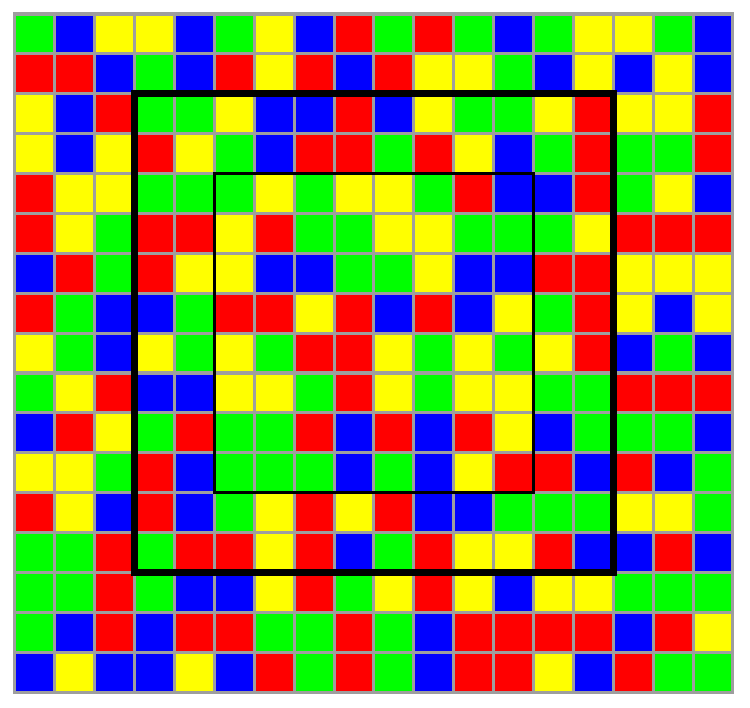
\includegraphics[width=0.45\textwidth]
{AKSs7colrBorderM1}\hspace{0.7cm}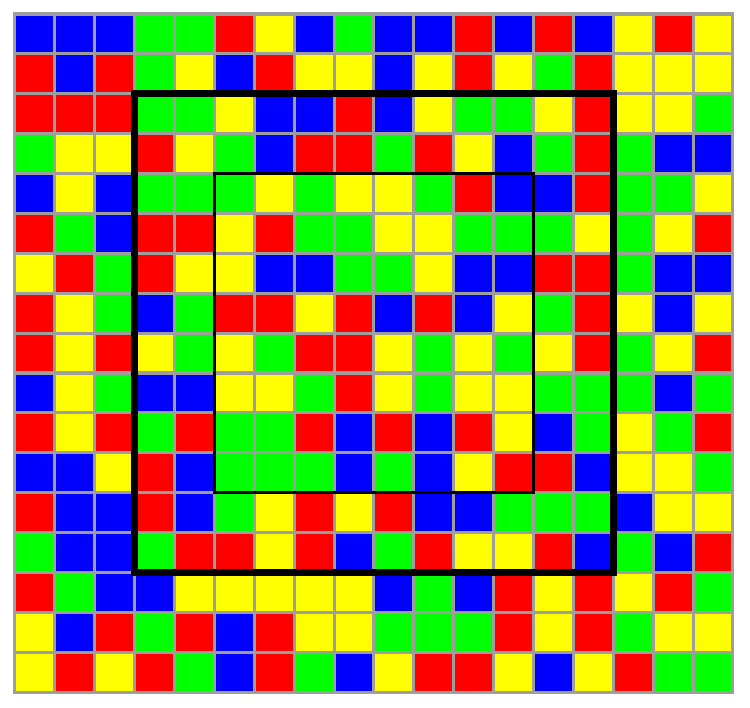
\includegraphics[width=0.45\textwidth]
{AKSs7colrBorderM2}
%{AKSs7BlockBorderM1}\hspace{0.7cm}\includegraphics[width=0.45\textwidth]
%{AKSs7BlockBorderM2}
\end{center}
%\caption[]{
2d symbolic representation of two {\twots}
shadowing each other within the shared
\brick\ $\Mm_{\R}=\Mm_{\R_{0}} \cup \Mm_{\R_{1}}$ % (blue)

\begin{itemize}
  \item border $\R_{1}$ (thick black), interior $\R_{0}$ (thin black)
  \item symbols outside \R\ differ
\end{itemize}
\vfill
$s=7$    \hfill                          Saremi 2017
%}
%\label{fig:AKScloseActSymb}
%\end{figure}
%%%%%%%%%%%%%%%%%%%%%%%%%%%%%%%%%%%%%%%%%%%%%%%%%%%%%%%%%%%%%%%%%%%%%%%
\end{frame}

\begin{frame}{solve}
\[
 (\Box -s+4)\ssp_{z} = \m_z
\] %\ee{LinearConn}
\begin{block}{Green's function $\gd$ for a $L\!\times\!T$ lattice}
yields the state $\ssp_{z}$ at every lattice point $z=\{\ell n\}$
\[
\ssp_{z} = \gd\,\m_z
\] %\ee{LinearConn}

\medskip
\end{block}
where
\[
\gd = \frac{1}{\Box -s+4}
\] %\ee{LinearConn}
is a Toeplitz (tensor) matrix, and \\
the integer $s$ is the local stretching rate \\
(how chaotic is each site)
\end{frame}

\begin{frame}{shadowing, \statesp}
%%%%%%%%%blogCats \label{fig:AKSs7dist} %%%%%%%%%%%%%%%%%%%%%%%%%%%%%
\begin{center}
(a) 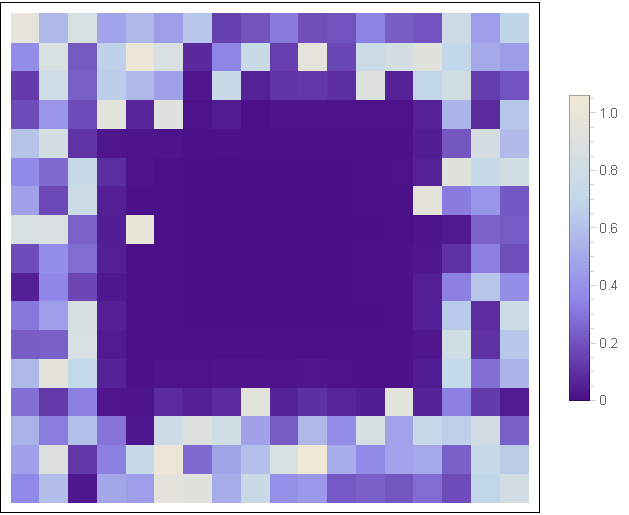
\includegraphics[width=0.40\textwidth]
{AKSs7distM1M2} %\hspace{0.7cm}
(b) 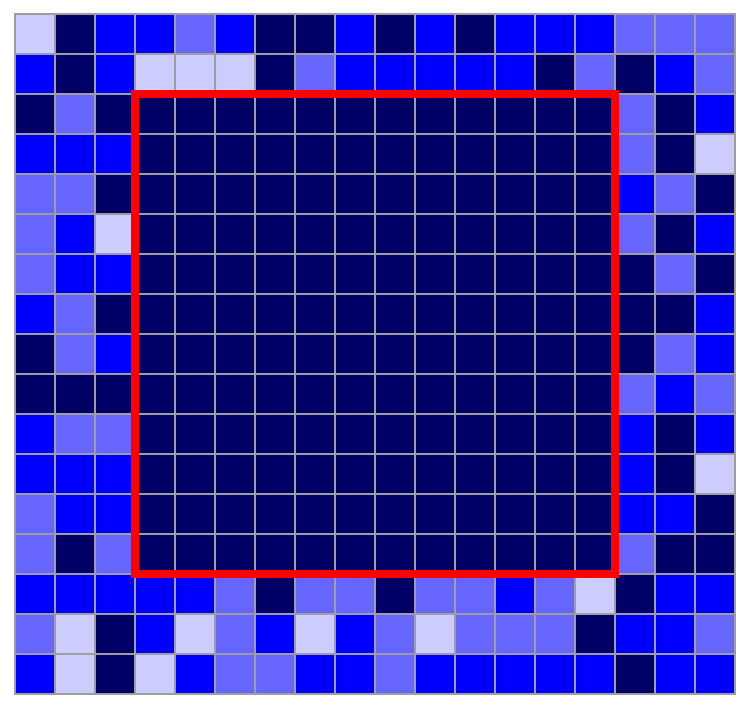
\includegraphics[width=0.35\textwidth]
{AKSs7distM1M2log}
\end{center}

\bigskip

(a)
\(
\Xx_{2,z}-\Xx_{1,z}
\,,
\)
the site-wise distance between the \twots\ fields corresponding to the
symbol \brick s
$\Mm_{1}$, $\Mm_{2}$ (colored tiles) previously
(left), respectively (right).

\medskip

(b)
The logarithm of the site-wise distance
\(
\ln|\Xx_{2,z}-\Xx_{1,z}|
\)
emphasizes the exponential falloff  of the distance around the center of the
shared \brick\ $\R=\R_{0} \cup \R_{1}$.

\vfill
\hfill                          Saremi 2018
\end{frame}


\begin{frame}{shadowing, \statesp}
$\Rightarrow$ within the interior of the shared \brick \\
the shadowing is \textcolor{blue}{exponentially close}
\end{frame}

\begin{frame}{this cat is}
\vfill
\begin{center}
{\huge chaotic}
\end{center}
\vfill
\end{frame}

\begin{frame}
 {the finest of chaotic field theories \\
  (superstringers, are you listening?) is}
%\begin{center}
%\hfill
\includegraphics[width=0.55\textwidth]{spatiotempCat}
\catlatt\hfill
\includegraphics[width=0.50\textwidth]{DawnBishopCats}
%\end{center}
\end{frame}

\begin{frame}{summary}
\begin{enumerate}
              \item
goal : describe states of turbulence in infinite spatiatemporal domains
              \item
victory if : can classify, enumerate all spatiotemporal tilings
              \item
the simplest model of ``turbulence'' : \catlatt
\end{enumerate}

\vfill

there is no more time

\medskip

there is only enumeration of admissible spacetime field configurations
\end{frame}

\begin{frame}{in future there will be no future}
\begin{center}
{\huge goodbye}
\end{center}

\vfill

to long time and/or space integrators

\medskip

\hfill they never worked and could never work
\end{frame}





\begin{frame}{XXX}
\end{frame}

\begin{frame}{XXX}
\end{frame}

\begin{frame}{XXX}
\end{frame}

\begin{frame}{XXX}
\end{frame}

\begin{frame}{XXX}
\end{frame}

\begin{frame}{take chronotopes to be spatiotemporally compact solutions}
\begin{center}
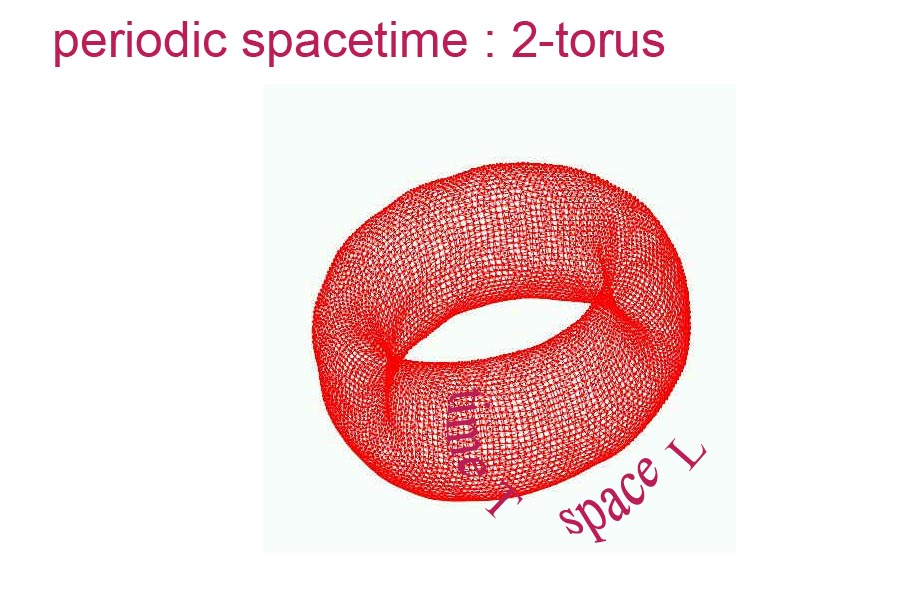
\includegraphics[width=0.9\textwidth]{torusSpTime}
\end{center}

\bigskip

after the space and time Fourier transforms, obtain
% \hfill \color{red}{(impossible without xxx)}
\end{frame}

\begin{frame}{there is no more space or time evolution}
a solution to \KS\ PDE \\
is now given as a condition that \\
at each lattice point $k\ell$ \\
the tangent field at $\Fu_{k\ell}$ \\
satisfies the equation of motion
\[
\left[- i \omega_\ell - ( q_k^2 - q_k^4 ) \right]\Fu_{k\ell}
+ i \frac{q_k}{2} \!\sum_{k'=0}^{N-1} \sum^{M-1}_{m'=0}\!\!
\Fu_{k'm'} \Fu_{k-k',m-m'}
    =
0
%\,.
%\label{e-FksSpattemp}
\]

\bigskip

this is a \textcolor{red}{local} tangent field constraint on a
\textcolor{red}{global} solution
\end{frame}

\begin{frame}{every calculation is a spatiotemporal lattice calculation}
field is discretized as
$\Fu_{k\ell}$ values  \\ over
$N M$ points of a periodic lattice

%\medskip

\begin{center}
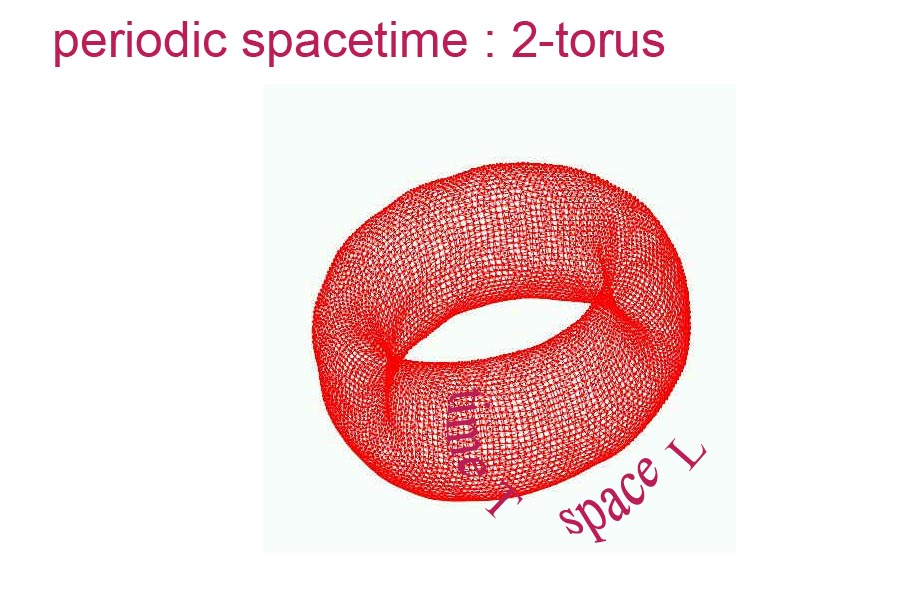
\includegraphics[width=0.9\textwidth]{torusSpTime}
\end{center}
% \hfill \color{red}{(impossible without xxx)}
\end{frame}

\begin{frame}{example : $s=3$ cat map symbolic dynamics}
%%%%%%%%%%%%%%%%%%%%%%%%%%%%%%%%%%%%%%%%%%%%%%%%%%%%%%%%%%%%%%%%
%\begin{figure}
  \begin{center}  %%% 2016-12-25  see
                  %%% siminos/figsSrc/inkscape/CatMapStatesp.svg
  \setlength{\unitlength}{0.55\textwidth}
 %% \unitlength = units used in the Picture Environment
  \begin{picture}(1,0.81984366)%
    \put(0,0){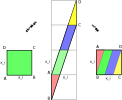
\includegraphics[width=\unitlength]{CatMapStatesp}}%
    \put(-0.025,0.15){\color[rgb]{0,0,0}\makebox(0,0)[lb]{\smash{}}}%
    \put(0.26669086,0.17307744){\color[rgb]{0,0,0}\makebox(0,0)[lb]{\smash{B}}}%
    \put(0.26669086,0.41839762){\color[rgb]{0,0,0}\makebox(0,0)[lb]{\smash{C}}}%
    \put(0.02137069,0.41839762){\color[rgb]{0,0,0}\makebox(0,0)[lb]{\smash{D}}}%
    \put(0.38935094,0.00135332){\color[rgb]{0,0,0}\makebox(0,0)[lb]{\smash{B}}}%
    %\put(0.32,0.17){\color[rgb]{0,0,0}\makebox(0,0)[lb]{\smash{$(0,0)$}}}%
    \put(0.64284833,0.60647641){\color[rgb]{0,0,0}\makebox(0,0)[lb]{\smash{C}}}%
    \put(0.64284833,0.79455521){\color[rgb]{0,0,0}\makebox(0,0)[lb]{\smash{D}}}%
    %\put(0.79004043,0.42657495){\color[rgb]{0,0,0}\makebox(0,0)[lb]{\smash{A}}}%
    %\put(0.79004043,0.17307744){\color[rgb]{0,0,0}\makebox(0,0)[lb]{\smash{B}}}%
    %\put(0.96994189,0.17307744){\color[rgb]{0,0,0}\makebox(0,0)[lb]{\smash{C}}}%
    %\put(0.97811923,0.42657495){\color[rgb]{0,0,0}\makebox(0,0)[lb]{\smash{D}}}%
    \put(0.02,0.27){\color[rgb]{0,0,0}\rotatebox{90.0}{\makebox(0,0)[lb]{\smash{$\ssp_{0}$}}}}%
    \put(0.39,0.27){\color[rgb]{0,0,0}\rotatebox{90.0}{\makebox(0,0)[lb]{\smash{$\ssp_{1}$}}}}%
    \put(0.76,0.27){\color[rgb]{0,0,0}\rotatebox{90.0}{\makebox(0,0)[lb]{\smash{$\ssp_{1}$}}}}%
    \put(0.1469525,0.16){\color[rgb]{0,0,0}\makebox(0,0)[lb]{\smash{$\ssp_{-1}$}}}%
    \put(0.51493279,0.16){\color[rgb]{0,0,0}\makebox(0,0)[lb]{\smash{$\ssp_{0}$}}}%
    \put(0.86655824,0.16){\color[rgb]{0,0,0}\makebox(0,0)[lb]{\smash{$\ssp_{0}$}}}%
    \put(0.21762677,0.55482852){\color[rgb]{0,0,0}\rotatebox{43.35476392}{\makebox(0,0)[lb]{\smash{stretch}}}}%
    \put(0.74915379,0.61465381){\color[rgb]{0,0,0}\rotatebox{-46.94301089}{\makebox(0,0)[lb]{\smash{wrap}}}}%
  \end{picture}%
\end{center}

%   \caption{ \label{fig:CatMapStatesp}
cat map stretches the unit square

translations by

\hfill $\Ssym{t} \in \A=\{\underline{1},0,1,2\}=$
\{%
{\color{red}red},
{\color{green}green},
{\color{blue}blue},
{\color{yellow}yellow}%
\}

return stray kittens back to the torus
\end{frame}

\begin{frame}{cat map $(\ssp_{0},\ssp_{1})$  \statesp\ partition}
%%%%%%%%%%%%%%%%%%%%%%%%%%%%%%%%%%%%%%%%%%%%%%%%%%%%%%%%%%%%%%%%%%
%\begin{figure}
\begin{center}
	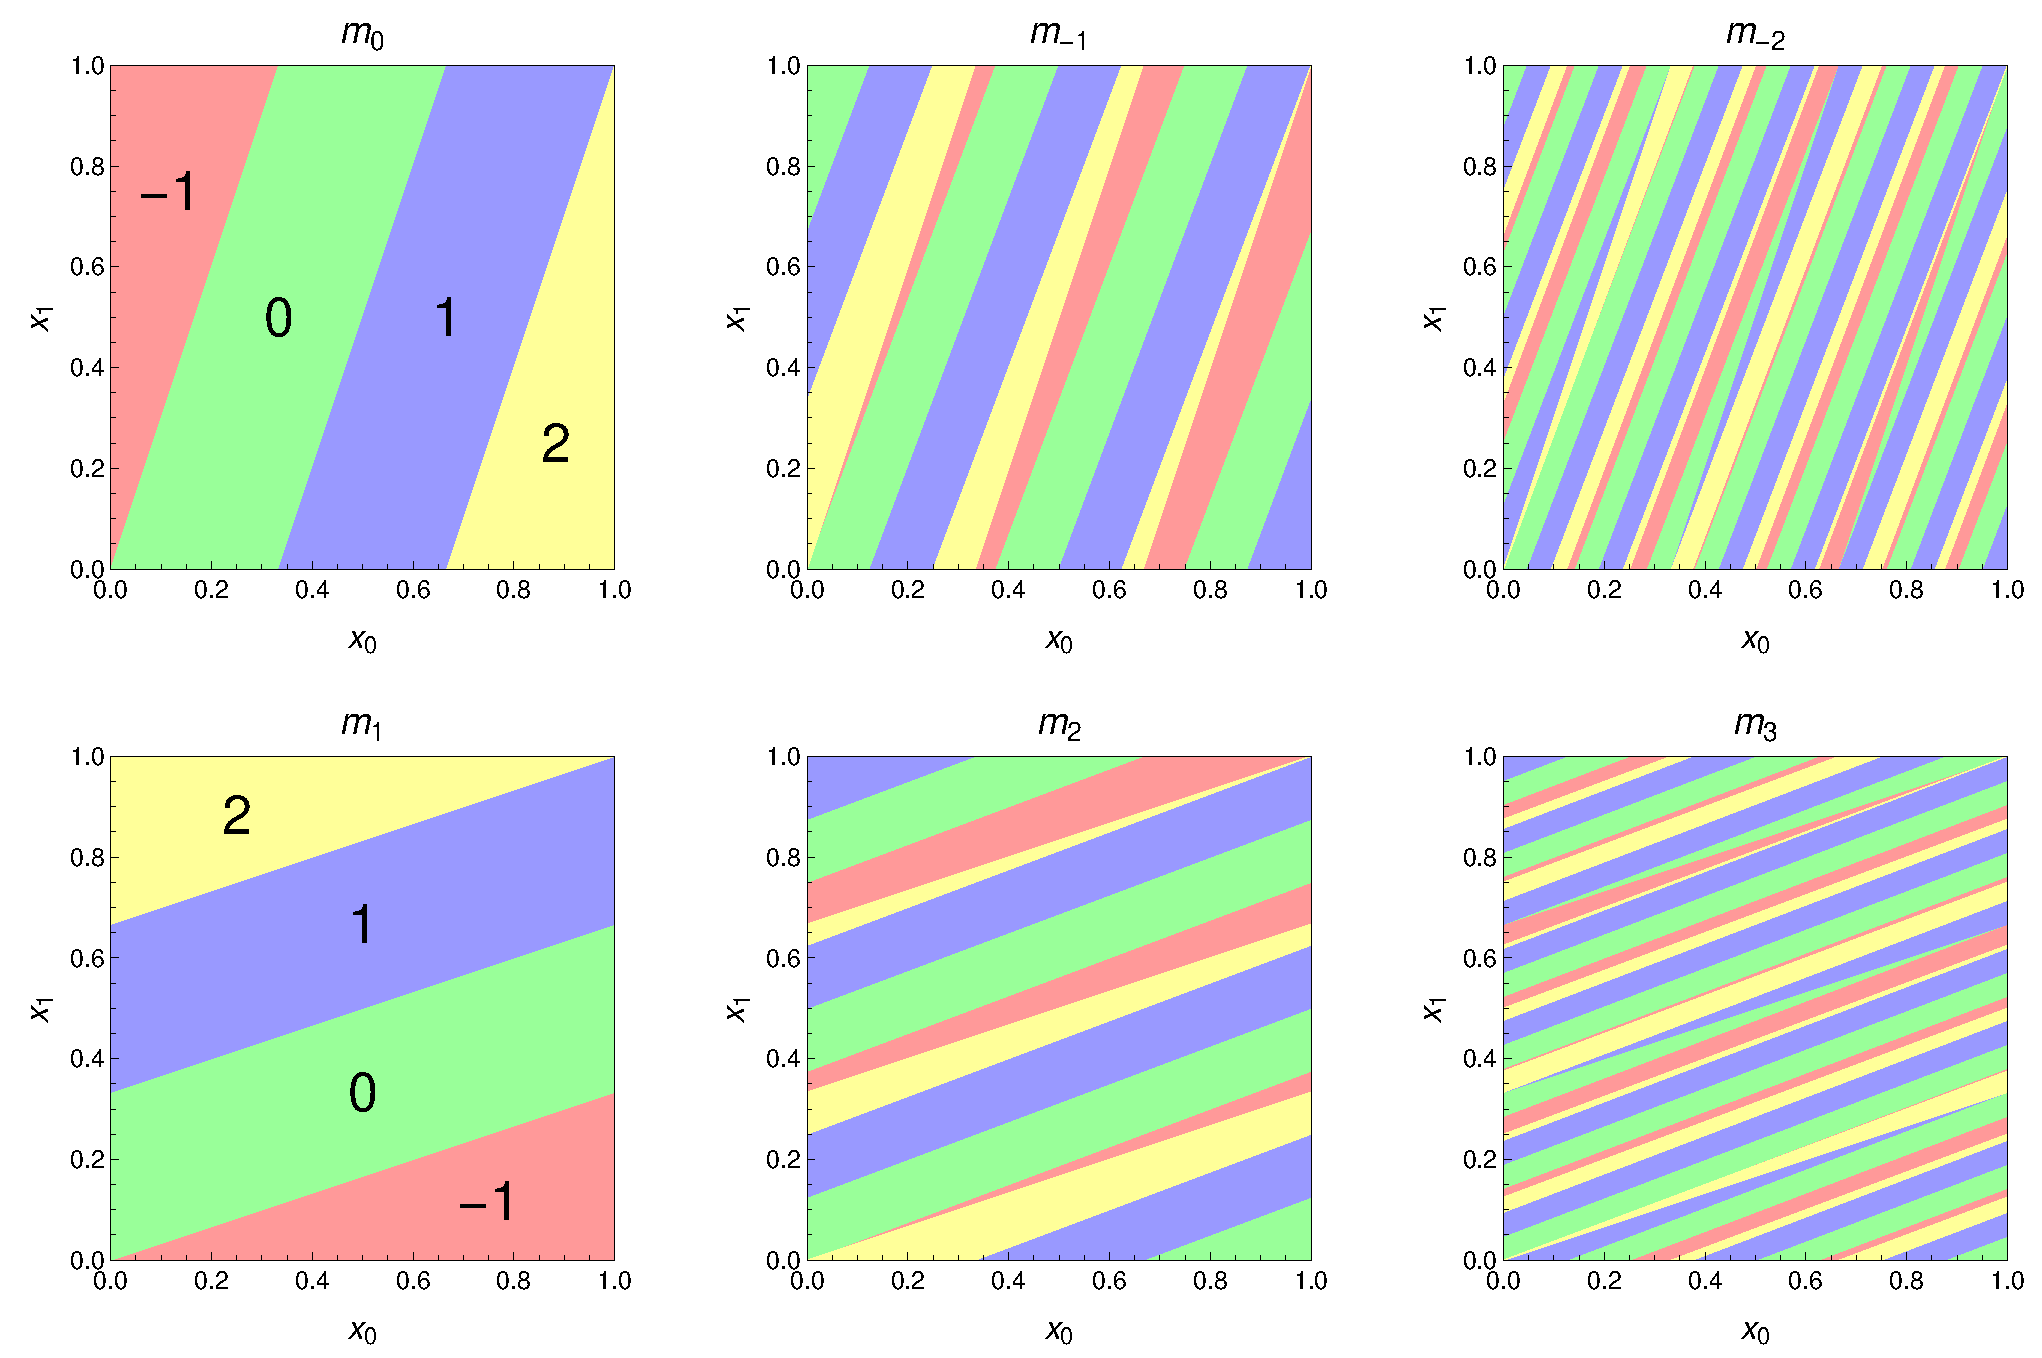
\includegraphics[width=0.75\textwidth]{SingleCat1Symbol}
\end{center}
%	\caption{\label{fig:SingleCat1color}

{\scriptsize
(a) 4 regions labeled by $\Ssym{0}.$ , obtained from
$(\ssp_{-1},\ssp_{0})$ \statesp\ by one iteration
\\
(b) 14 regions, 2-steps past $\Ssym{-1}\Ssym{0}.$
(c) 44 regions, 3-steps past $\Ssym{-2}\Ssym{-1}\Ssym{0}.$

\medskip

(d) 4 regions labeled by future $.\Ssym{1}$
\\
(e) 14 regions, 2-steps  future $.\Ssym{1}\Ssym{2}$
(f) 44 regions, 3-steps future {\brick} $\Ssym{3}\Ssym{2}\Ssym{1}.$
}
%\end{figure}
%%%%%%%%%%%%%%%%%%%%%%%%%%%%%%%%%%%%%%%%%%%%%%%%%%%%%%%%%%%%%%%%%%
\end{frame}

\begin{frame}{Percival-Vivaldi unit square is \textcolor{red}{not} a partition}
%%%%%%%%%%%%%%%%%%%%%%%%%%%%%%%%%%%%%%%%%%%%%%%%%%%%%%%%%%%%%%%%
%\begin{figure}
  \begin{center}  %%% 2016-12-25  see
                  %%% siminos/figsSrc/inkscape/CatMapStatesp.svg
  \setlength{\unitlength}{0.55\textwidth}
 %% \unitlength = units used in the Picture Environment
  \begin{picture}(1,0.81984366)%
    \put(0,0){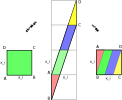
\includegraphics[width=\unitlength]{CatMapStatesp}}%
    \put(-0.025,0.15){\color[rgb]{0,0,0}\makebox(0,0)[lb]{\smash{}}}%
    \put(0.26669086,0.17307744){\color[rgb]{0,0,0}\makebox(0,0)[lb]{\smash{B}}}%
    \put(0.26669086,0.41839762){\color[rgb]{0,0,0}\makebox(0,0)[lb]{\smash{C}}}%
    \put(0.02137069,0.41839762){\color[rgb]{0,0,0}\makebox(0,0)[lb]{\smash{D}}}%
    \put(0.38935094,0.00135332){\color[rgb]{0,0,0}\makebox(0,0)[lb]{\smash{B}}}%
    %\put(0.32,0.17){\color[rgb]{0,0,0}\makebox(0,0)[lb]{\smash{$(0,0)$}}}%
    \put(0.64284833,0.60647641){\color[rgb]{0,0,0}\makebox(0,0)[lb]{\smash{C}}}%
    \put(0.64284833,0.79455521){\color[rgb]{0,0,0}\makebox(0,0)[lb]{\smash{D}}}%
    %\put(0.79004043,0.42657495){\color[rgb]{0,0,0}\makebox(0,0)[lb]{\smash{A}}}%
    %\put(0.79004043,0.17307744){\color[rgb]{0,0,0}\makebox(0,0)[lb]{\smash{B}}}%
    %\put(0.96994189,0.17307744){\color[rgb]{0,0,0}\makebox(0,0)[lb]{\smash{C}}}%
    %\put(0.97811923,0.42657495){\color[rgb]{0,0,0}\makebox(0,0)[lb]{\smash{D}}}%
    \put(0.02,0.27){\color[rgb]{0,0,0}\rotatebox{90.0}{\makebox(0,0)[lb]{\smash{$\ssp_{0}$}}}}%
    \put(0.39,0.27){\color[rgb]{0,0,0}\rotatebox{90.0}{\makebox(0,0)[lb]{\smash{$\ssp_{1}$}}}}%
    \put(0.76,0.27){\color[rgb]{0,0,0}\rotatebox{90.0}{\makebox(0,0)[lb]{\smash{$\ssp_{1}$}}}}%
    \put(0.1469525,0.16){\color[rgb]{0,0,0}\makebox(0,0)[lb]{\smash{$\ssp_{-1}$}}}%
    \put(0.51493279,0.16){\color[rgb]{0,0,0}\makebox(0,0)[lb]{\smash{$\ssp_{0}$}}}%
    \put(0.86655824,0.16){\color[rgb]{0,0,0}\makebox(0,0)[lb]{\smash{$\ssp_{0}$}}}%
    \put(0.21762677,0.55482852){\color[rgb]{0,0,0}\rotatebox{43.35476392}{\makebox(0,0)[lb]{\smash{stretch}}}}%
    \put(0.74915379,0.61465381){\color[rgb]{0,0,0}\rotatebox{-46.94301089}{\makebox(0,0)[lb]{\smash{wrap}}}}%
  \end{picture}%
\end{center}
%   \caption{ \label{fig:CatMapStatesp}
forward iteration of the unit square yields a grammar with infinity of
longer and longer inadmissible sequences (pruning rules)

\bigskip
\hfill that's stupid
\end{frame}

\begin{frame}{
spacetime lattice sites $z=(\conf,\zeit) \in (-\infty, \infty)\times (-\infty, \infty)$
             }

\bigskip

continuous symmetries : space, time translations
\medskip

\begin{center}
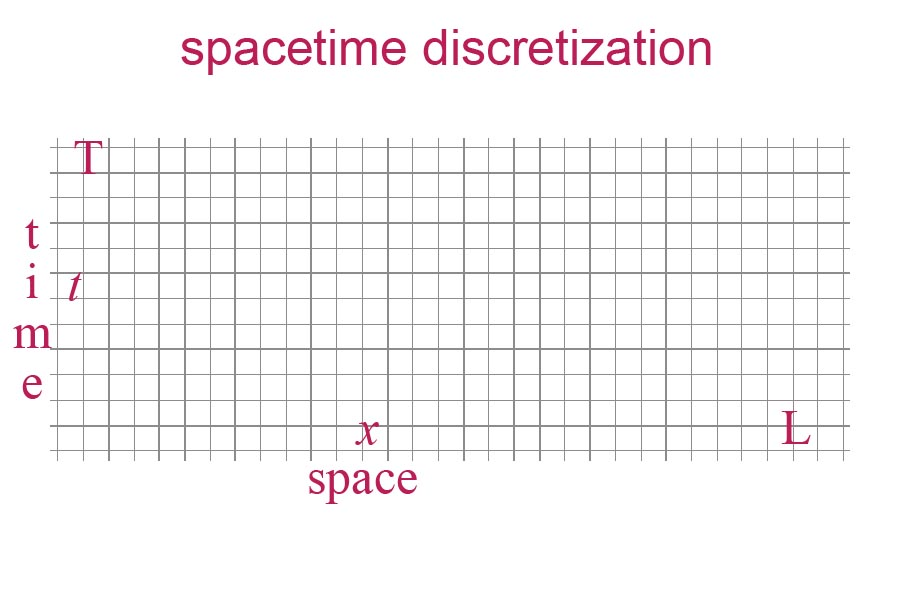
\includegraphics[width=1.1\textwidth]{spaceTime}
\end{center}
% \hfill \color{red}{(impossible without xxx)}
\end{frame}

\begin{frame}{
the 3-letter translations alphabet \;+\; the Markov graph
             }

\medskip

generates the admissible orbits
\beq
\Ssym{t}\in\{\underline{1},0,1\}
\ee{threeLett}
example : all admissible 4-cycles
\bea
{\bf x}_{0 0 1 \underline{1}} &=& \frac{1}{15}
\left[
\begin{array}{cccc}
 {-1} &
 {1} &
 {4} &
 {-4}
\end{array}
\right]
    \,,\qquad
{\bf x}_{0 1 0 \underline{1}}= \frac{1}{15}
\left[
\begin{array}{cccc}
 {0} &
 {5} &
 {0} &
 {-5}
\end{array}
\right]
    \continue
{\bf x}_{0 1 \underline{1}1} &=& \frac{1}{15}
\left[
\begin{array}{cccc}
 {4} &
 {6} &
 {-1} &
 {6}
\end{array}
\right]
    \,,\qquad
{\bf x}_{0 1 1 \underline{1}}= \frac{1}{15}
\left[
\begin{array}{cccc}
 {2} &
 {8} &
 {7} &
 {-2}
\end{array}
\right]
    \continue
% Predrag 2018-02-19 replaced the
% old 6 \cycle{3125} \\  1 0 1 \underline{1} = 4 \cycle{1253}
% by new No. 6:
% 6 \cycle{1133} \\  0 0 1            1
{\bf x}_{0 0 1 1} &=& \frac{1}{15}
\left[
\begin{array}{cccc}
 {5} &
 {5} &
 {10} &
 {10}
\end{array}
\right]
    \,,\qquad
{\bf x}_{1 1 1 \underline{1}}= \frac{1}{15}
\left[
\begin{array}{cccc}
 {9} &
 {11} &
 {9} &
 {1}
\end{array}
\right]
    \continue
{\bf x}_{1 1 1 0} &=& \frac{1}{15}
\left[
\begin{array}{cccc}
 {12} &
 {13} &
 {12} &
 {8}
\end{array}
\right]
    \,,\qquad
{\bf x}_{1 1 0 \underline{1}}= \frac{1}{15}
\left[
\begin{array}{cccc}
 {7} &
 {8} &
 {2} &
 {-2}
\end{array}
\right]
    \continue
{\bf x}_{0 0 \underline{1}1} &=& \frac{1}{15}
\left[
\begin{array}{cccc}
 {1} &
 {-1} &
 {-4} &
 {4}
\end{array}
\right]
\label{4cyclesPerPoints}
\eea
\end{frame}

\begin{frame}{example : all admissible 4-cycles}
\begin{center}
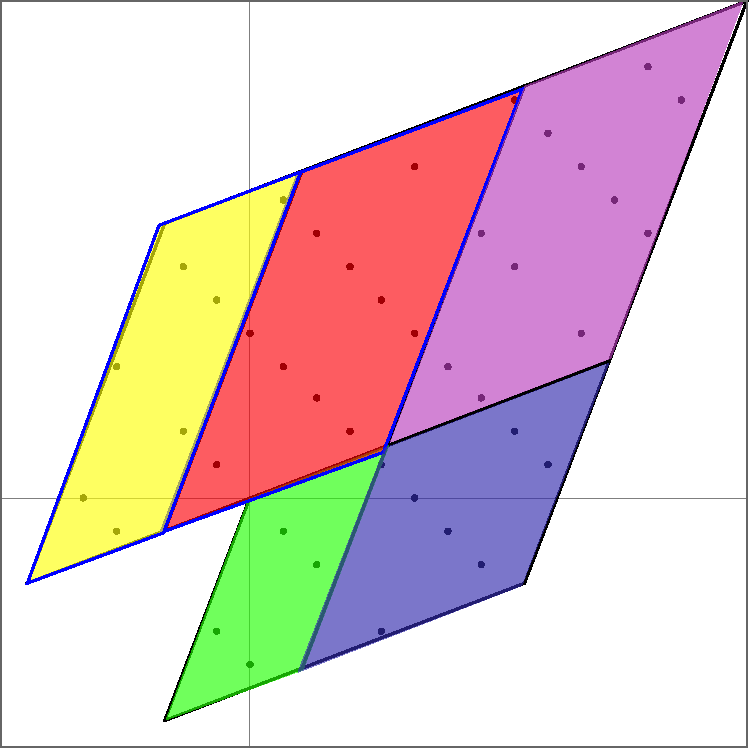
\includegraphics[width=0.40\textwidth]{HLAllCyclePointsB}
\end{center}


%  \caption{\label{fig:HLAllCyclePoints}
All prime 4-cycles periodic points fit snugly into the partition

%\medskip
%The holes correspond to missing cycle-1 and cycle-2 points.
\end{frame}

\begin{frame}{chronotope
    \footfullcite{LePoTo96}%$^,$\footfullcite{WK09}
}
\begin{bartlett}{
the chronotope is how a
configuration of time and space is represented in language and
discourse.
                }\bauthor{
\HREF{https://en.wikipedia.org/wiki/Chronotope}
{Wikipedia : Chronotope}
                }
\end{bartlett}

\bigskip
\bigskip
%goes without saying : was done by a Soviet scientist first

\begin{itemize}
  \item Mikhail Mikhailovich Bakhtin (1937)
%  \item Politi, Giacomelli, Lepri, Torcini (1996)
%  \item Gutkin and Osipov (2016)
\end{itemize}
\end{frame}

\end{document}
